\documentclass[11pt,a4paper,titlepage]{article}
\usepackage{amsmath,amssymb,amstext,amsfonts,mathrsfs,graphicx}
\begin{document}
\title{GEP Protokoll - Laborversuch 5\\
Oszilloskop 2}
\author{Cao Thi Huyen \and Robert R\"osler \and Nico Grimm}
\date{7. Dezember 2015}
\maketitle
\section{Scheinwiderstandsmessung}
Mit einem Oszilloskop ist durch gleichzeitige Strom- und Spannungsmessung eine komplexe Impedanz \((\underline{Z}=R+j\omega L)\) einer Spule (0.1H, 10$\Omega$) zu bestimmen.
\subsection{Messaufbau}
Um den Spulenstrom mit dem Oszillioskop messen zu k\"onnen, wird der Spule ein geeigneter Widerstand (50$\Omega$) vorgeschaltet. Der Strom wird dann indirekt \"uber den Spannungsabfall an diesem Vorwiderstand bestimmt. Am Signalgenerator wird eine Frequenz von 50Hz (Sinus) eingestellt.
\begin{center}
Platzhalter f\"ur den Schaltplan
\end{center}
\subsection{Ergebnisse}
\subsubsection{Dokumentation der Zeitfunktionen von Strom und Spannung in DC-Kopplung}
\begin{figure}[h!]
\label{fig:aufg1}
\begin{center}
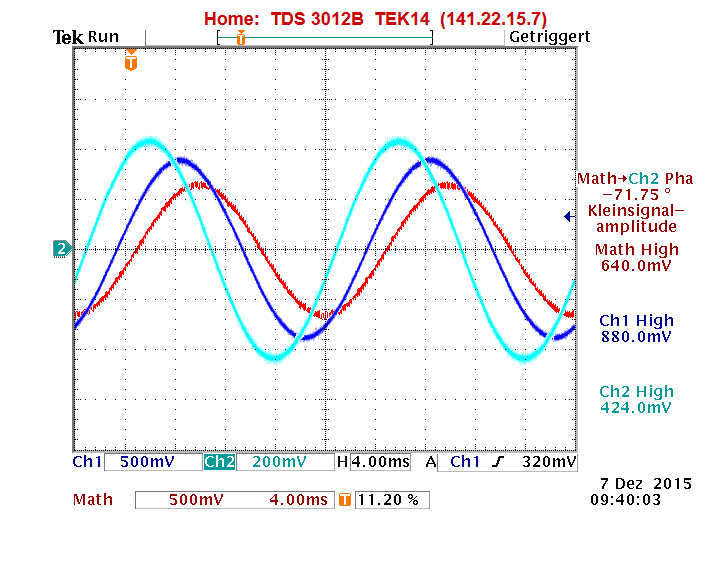
\includegraphics[width=0.9\textwidth]{5_1_1}
\end{center}
\end{figure}
Channel 1 (hier dunkelblau) stellt die Spannung dar, die \"uber dem Vorwiderstand abf\"allt. Channel 2 (hier hellblau) stellt die Spannung \"uber der Spule dar. Der Gesamtstrom der flie\ss{}t, wird durch die Subtraktion von Channel 2 und Channel 1 rechnerisch dargestellt.
\newpage
\subsubsection{Berechnung der Impedanz \underline{Z} und Bestimmung der Bauelementgr\"o\ss{}en}
Messwerte die aus \ref{fig:aufg1} entnommen sind und zur Berechnung ben\"otigt werden sind:
\begin{itemize}
\item Phasenverschiebung $\varphi = -71.75^\circ$
\item \^u = 880mV
\item \(\hat{i} = \frac{u_x}{R_1}$ mit $u_x = 640mV$, daraus folgt $\hat{i} = \frac{8}{625}A\) 
\end{itemize}  
Aus diesen Werten l\"asst sich die Impedanz \underline{Z} und die daraus resultierenden Bauelementgr\"o\ss{}en R und L berechnen. \\[1ex]
\(\underline{Z} = \frac{\hat{u}}{\hat{i}} \cdot e^{-j71.75} \Rightarrow \underline{Z} = 68.75\Omega \cdot e^{j71.75}\) \\[1ex]
$\Rightarrow \underline{Z} = 21.5\Omega + j65.3\Omega$ \\[1ex]
Hier k\"onnen wir unserern gesuchten Widerstand R einfach ablesen: R = 21,5$\Omega$ \\[1ex]
Da der Strom nacheilt, handelt es sich im Induktivit\"at! \\[1ex]
$\omega \cdot L = 65.3\Omega \Leftrightarrow L = \frac{65.3\Omega}{2\pi50Hz} = 0.2H$ \\[1ex]
Somit haben wir die Bauelementgr\"o\ss{}en mit R = 21.5$\Omega$ und L = 0.2H bestimmt!
\newpage
\section{Messung der Kennlinie eines VDR im X-Y-Betrieb}
Ziel der Messung ist die ma\ss{}stabsgerechte Darstellung der u = f(i)-Kennlinie eines spannungsabh\"angigen Widerstandes (VDR) bei 50Hz (aus Stelltrenntrafo). Es wird dabei auf einen maximalen Strom von 125mA geachtet. Auf dem Oszilloskop soll u = f(i) wie folgt dargestellt werden: \\[1ex] 
"i" wird in x-Richtung und "u" in y-Richtung dargestellt \\

\underline{Kennliniengleichung des VDR:} \\[1ex]
\begin{equation}\label{vdr}
\frac{u}{V}=C\cdot(\frac{i}{mA})^{\beta} mit \beta = 0.36 und C = 1.75 
\end{equation}
\subsubsection*{Die Kennlinie wird mit folgender Schaltung gemessen}
\begin{center}
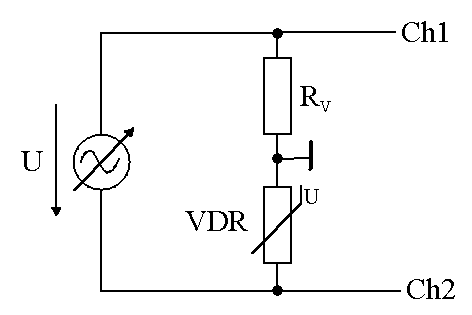
\includegraphics[width=0.7\textwidth]{gep2v5_2}
\end{center}
Der Widerstand $R_V$ wird mit 40$\Omega$ dimensioniert. Hierbei betr\"agt der Spannungsabfall genau 1V bei einem Strom von 25mA.
\newpage
\subsection{Vergleich: Berechnung und Messung bei i = 100mA}
\subsubsection{Berechnung der Spannung $u_1$}
Nach \eqref{vdr} mit $i = 100mA \to u = \sim9.18V$
\subsubsection{Messung von $u_1$, $R_1$ und $r_1$} 
\begin{center}
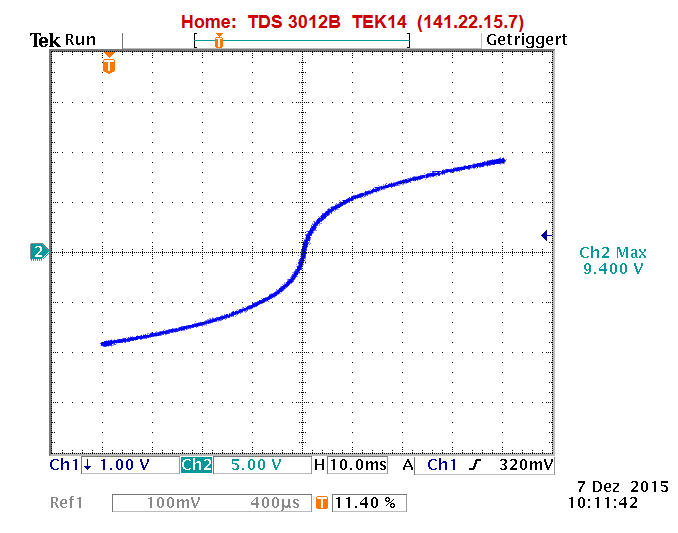
\includegraphics[width=0.8\textwidth]{5_2_1}
\end{center}
Die Spannung $u_1$ k\"onnen wir am Graphen beim Stromwert $i_1 = 100mA$ ablesen. \\[1ex]
$u_1 = \sim 9V$ \\[1ex]
Der Widerstand $R_1$ wird durch die Formel $R=\frac{u_1}{i_1}$ berechnet. \\[1ex]
$R=\frac{9V}{100mA}=90\Omega$ \\[1ex]
Den differentiellen Widerstand $r_1$ bestimmen wir durch eine Tangente durch die beiden Punkte \{(100mA, 9V), (75mA, 8V)\}. \\[1ex]
Daraus ergibt sich ein differentieller Widerstand $r_1 = 40\Omega$
\newpage
\subsubsection{Kopplungsart AC/DC}
\begin{center}
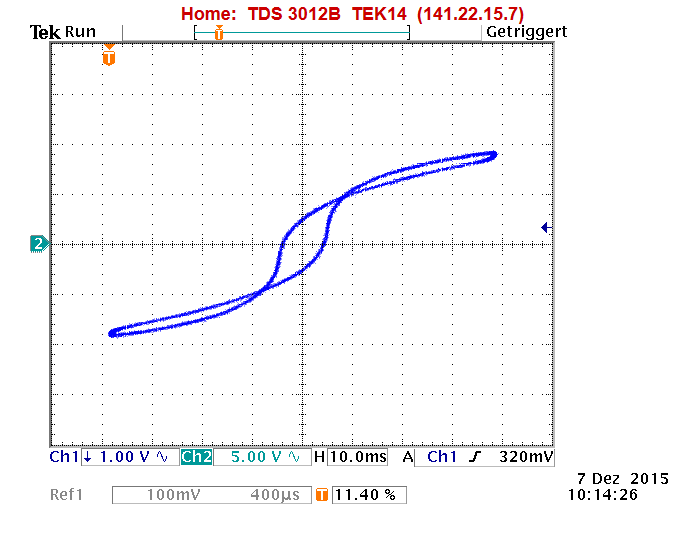
\includegraphics[width=0.8\textwidth]{5_2_2}
\end{center}
Anhand der gezeigten Ausgabe am Oszilloskop ist zu best\"atigen, dass eine \"Anderung der Kopplungsart von Gleischstrom auf Wechselstrom einen Einfluss auf die Eingangsschaltung des Oszilloskops hat.
\end{document}
